\documentclass[12pt,addpoints]{evalua}
\grado{1$^\circ$ de Secundaria}
\cicloescolar{2023-2024}
\materia{Matemáticas 1}
\unidad{3}
\title{Examen de la Unidad}
\aprendizajes{\footnotesize%
    \item Verifica algebraicamente la equivalencia de expresiones de primer grado, formuladas a partir de sucesiones.
    \item Resuelve problemas mediante la formulación y solución algebraica de ecuaciones lineales.
    \item Usa e interpreta las medidas de tendencia central (moda, media aritmética y mediana).
    \item Calcula el área y volumen de piramides, prismas y cilindros rectos.
    \item Calcula el perímetro y el área de polígonos regulares y del círculo a partir de diferentes datos.
    }
     \author{Prof.: Julio César Melchor Pinto}
\begin{document}
\begin{questions}

      \question[6]{Escribe los términos faltantes de las siguientes sucesiones aritméticas:

            \begin{multicols}{3}
                  \begin{parts}
                        \part 21, 25, 29, \fillin[33][0.5cm], \fillin[37][0.5cm], \fillin[41][0.5cm], \dots
                        % \part  4, 10, 16, \fillin[22][0.5cm], \fillin[28][0.5cm], \fillin[34][0.5cm], \dots
                        % \part 34, 31, 28, \fillin[25][0.5cm], \fillin[22][0.5cm], \fillin[19][0.5cm], \dots
                        % \part 92, 86, 80, \fillin[74][0.5cm], \fillin[68][0.5cm], \fillin[62][0.5cm], \dots
                        \part 51, 46, 41, \fillin[36][0.5cm], \fillin[31][0.5cm], \fillin[26][0.5cm], \dots
                        \part 250,225,200, \fillin[175][0.5cm], \fillin[150][0.5cm], \fillin[125][0.5cm], \dots
                  \end{parts}
            \end{multicols}
      }

      % \subsection*{Completa la sucesión aritmética 2}



      \question[6]{Escribe los primeros 4 términos de las siguientes sucesiones aritméticas:

            \begin{multicols}{3}
                  \begin{parts}
                        \part $a_n=7n+4$ \\ \fillin[11][0.5cm], \fillin[18][0.5cm], \fillin[25][0.5cm], \fillin[32][0.5cm], \dots
                        \part $a_n=-5n+15 $ \\  \fillin[10][0.5cm], \fillin[5][0.5cm], \fillin[0][0.5cm], \fillin[-5][0.5cm], \dots
                        \part $a_n=-n-5$  \\  \fillin[-6][0.5cm], \fillin[-7][0.5cm], \fillin[-8][0.5cm], \fillin[-9][0.5cm], \dots
                  \end{parts}
            \end{multicols}
      }

      \subsection*{Completa la sucesión geométrica}


      \question[6]{Escribe los términos faltantes de las siguientes sucesiones geométricas

            \begin{multicols}{3}
                  \begin{parts}
                        \part 12, 60, \fillin[300][0.8cm], \fillin[1500][0.8cm], \fillin[7500][0.8cm], \dots
                        \part 10, 20, \fillin[40][0.8cm], \fillin[80][0.8cm], \fillin[160][0.8cm], \dots
                        \part 2, 4, 8 \fillin[16][0.5cm], \fillin[32][0.5cm], \fillin[64][0.5cm], \dots
                  \end{parts}
            \end{multicols}
      }

      \subsection*{Diferencia de una sucesión}

      \question[6]{Determina la diferencia de las siguientes sucesiones aritméticas:

            \begin{multicols}{3}
                  \begin{parts}
                        \part 14, 12, 10, 8, 6, \dots \\[0.5em]
                        d=\fillin[-2][1cm]
                        \part 33, 27, 21, 15, 9, \dots \\[0.5em]
                        d=\fillin[-6][1cm]
                        \part -10, -8, -6, -4,  \dots \\[0.5em]
                        d=\fillin[2][1cm]
                  \end{parts}
            \end{multicols}
      }

      \subsection*{Término de una sucesión}


      \question[4]{
            \begin{multicols}{2}
                  \begin{parts}
                        \part ¿Cuál es el término 29 de la siguiente sucesión?

                        $a_{n}=12n+24$

                        \begin{solutionbox}{1.3cm}
                              $a_{29}=12(29)+24=372$
                        \end{solutionbox}

                        \part ¿Cuál es el término 41 de la siguiente sucesión?

                        $a_{n}=5n+5$

                        \begin{solutionbox}{1.3cm}
                              $a_{41}=5(41)+5=210$
                        \end{solutionbox}
                  \end{parts}
            \end{multicols}
      }

      \section*{Proporcionalidad y estadística}
      \subsection*{Razones y proporciones}



      \question[8]{Resuelve los siguientes problemas:

            \begin{multicols}{2}
                  \begin{parts}
                        \part Si la razón entre niños y niñas en un salón es de 2 a 3, ¿cuántas niñas habrá en un salón en donde hay 25 personas?
                        \fillin[10][2cm]
                        \begin{solutionbox}{1.5cm}
                        \end{solutionbox}

                        \part El costo de un kilo de aguacate es de 68 pesos, ¿cuánto se pagará por cinco cajas que cada una tiene 16 kilos de aguacate?
                        \fillin[5440][2cm]
                        \begin{solutionbox}{1.5cm}
                        \end{solutionbox}

                        %         \end{parts}
                        %     \end{multicols}
                        % }


                        %\subsection*{Variación directa e inversa}

                        % \question[4]{Contesta las siguientes preguntas:

                        %     \begin{multicols}{2}
                        %         \begin{parts}
                        \part Si 12 vacas se comen un granero lleno de paja en 80 días, ¿cuánto tardarán en comerse la misma cantidad de paja 30 vacas?
                        \fillin[32][2cm]
                        \begin{solutionbox}{1.5cm}
                        \end{solutionbox}

                        \part Si para pintar 180 metros de pared se necesitan 24 litros de pintura, ¿cuántos litros se necesitarán para pintar 270 metros de pared?
                        \fillin[36][2cm]
                        \begin{solutionbox}{1.5cm}
                        \end{solutionbox}

                  \end{parts}
            \end{multicols}
      }


      \subsection*{Mediana y moda}



      \question[4]{Contesta las siguientes preguntas:

            \begin{multicols}{2}
                  \begin{parts}
                        \part Las calificaciones de un salón de secundaria son las siguientes: 5, 7, 6, 8, 7, 9, 10, 7, 8, 7, 9, 7. ¿Cuál es la mediana de las calificaciones?
                        \fillin[7][2cm]
                        \begin{solutionbox}{2cm}
                        \end{solutionbox}

                        \part Las edades de un grupo de personas son: 15, 17, 15, 18, 19, 14, 15, 13 y 17 años. ¿Cuál es la mediana de las edades?
                        \fillin[15][2cm]
                        \begin{solutionbox}{2cm}
                        \end{solutionbox}

                  \end{parts}
            \end{multicols}
      }

      % \ejemplosboxed[{En mi colegio entre alumnos y alumnas somos 418. Si el número de chicas supera en 42 al de chicos, ¿cuántos alumnos y alumnas hay?

      %                   \begin{solutionbox}{1.5cm}
      %                   \end{solutionbox}
      %             }]

      % \question[6]{En mi colegio entre alumnos y alumnas somos 418. Si el número de chicas supera en 42 al de chicos, ¿cuántos alumnos y alumnas hay?

      %       \begin{solutionbox}{1.5cm}
      %       \end{solutionbox}
      % }

      \newpage
      \subsection*{Promedio}

      \question[4]{Contesta las siguientes preguntas:

            \begin{multicols}{2}
                  \begin{parts}
                        \part Las estaturas de un grupo de personas son: 171, 172, 168, 166, 164, 178 y 175 cm, ¿cuál es el promedio de la estatura de las personas?
                        \fillin[170.57][2cm]
                        \begin{solutionbox}{1.5cm}

                        \end{solutionbox}

                        \part En un grupo de 9 personas se registraron los siguientes pesos: 87, 60, 71, 74, 81, 80, 66, 74 y 79 kg. ¿Cuál es el promedio de los pesos?
                        \fillin[74.66][2cm]
                        \begin{solutionbox}{1.5cm}
                        \end{solutionbox}

                  \end{parts}
            \end{multicols}
      }

      \subsection*{Interpretación de gráficas}



      \question[3]{Los resultados de una encuesta se muestran en la siguiente gráfica de barras:

            \begin{multicols}{2}
                  \begin{parts}
                        \part  ¿Cuántas personas participaron en la encuesta? \fillin[95][2cm]
                        \part  ¿Cuál es la fruta menos preferida por las personas? \fillin[Naranja][2cm]
                        \part  ¿Cuál es la fruta preferida por las personas? \fillin[Manzana][2cm]

                        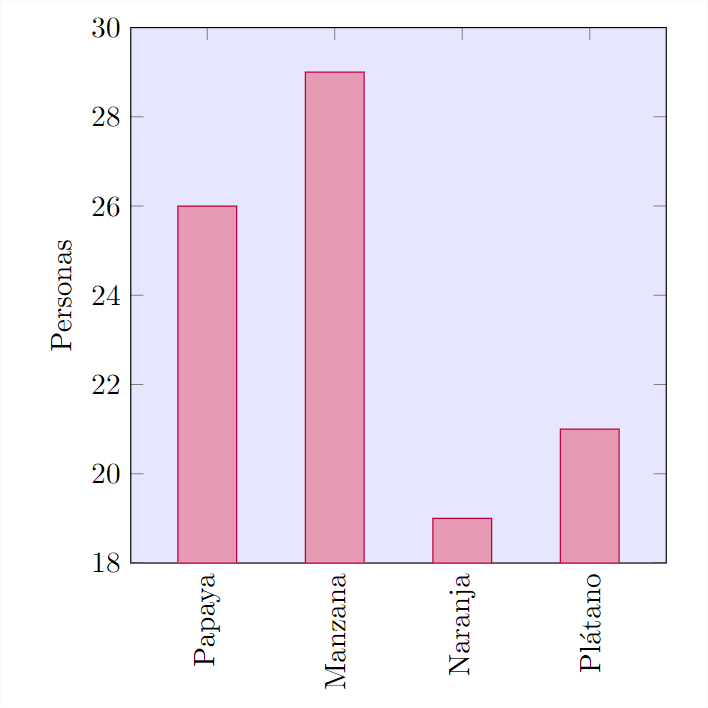
\includegraphics[width=.7\linewidth]{mexmat00001.png}
                  \end{parts}
            \end{multicols}

      }

      % \newpage

      \section*{Círculo}
      \subsection*{Diámetro, Radio. Perímetro y Área de un círculo}


      \question[9]{ Calcula el perímetro y área de los siguientes círculos:

            \begin{multicols}{3}
                  \begin{parts}
                        \part 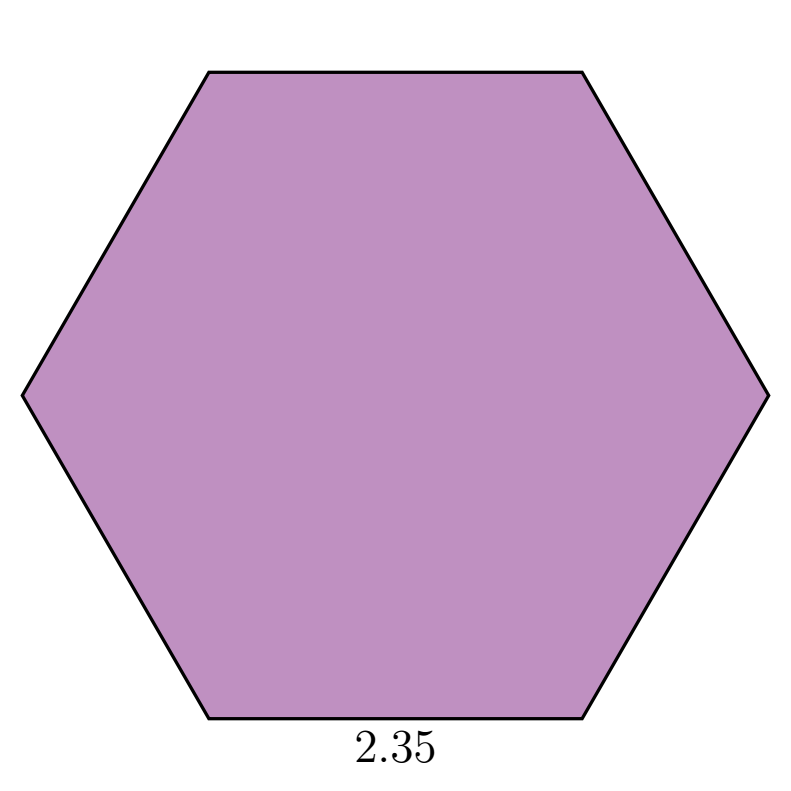
\includegraphics[width=0.85\linewidth]{mex_0007.png}\\
                        Perímetro: \fillin[][0.3in] \quad Área: \fillin[][0.3in]
                        \begin{solutionbox}{2cm}
                        \end{solutionbox}
                        \part 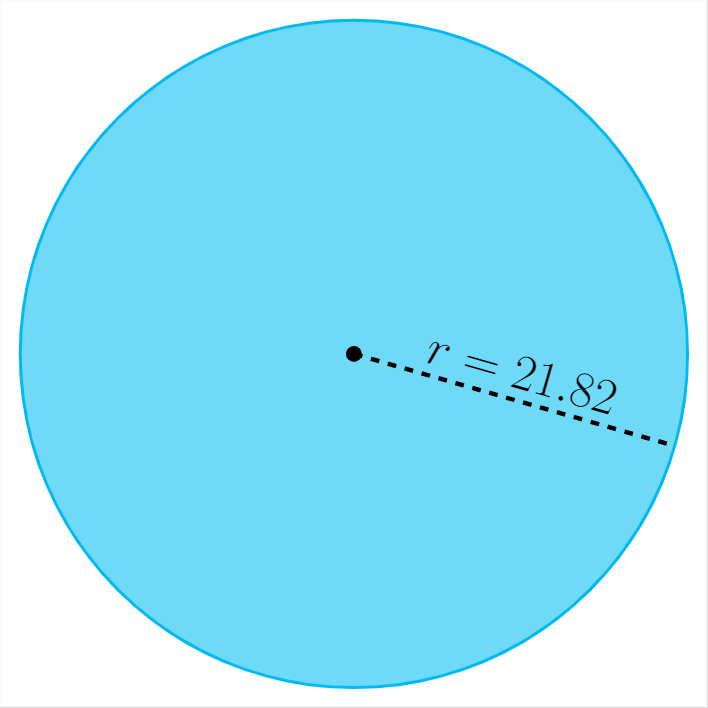
\includegraphics[width=0.85\linewidth]{mex_0008.png}\\
                        Perímetro: \fillin[][0.3in] \quad Área: \fillin[][0.3in]
                        \begin{solutionbox}{2cm}
                        \end{solutionbox}
                        \part 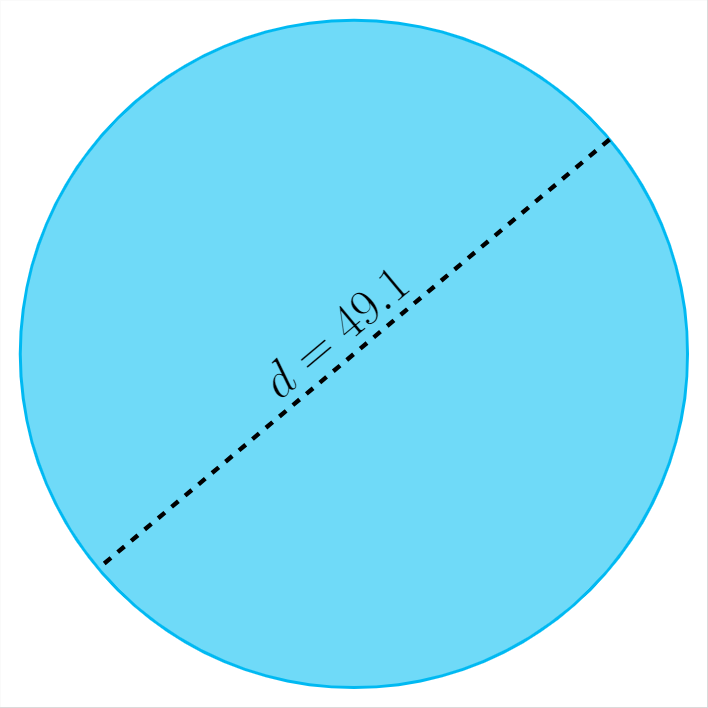
\includegraphics[width=0.85\linewidth]{mex_0009.png}\\
                        Perímetro: \fillin[][0.3in] \quad Área: \fillin[][0.3in]
                        \begin{solutionbox}{2cm}
                        \end{solutionbox}
                  \end{parts}
            \end{multicols}

      }

      \subsection*{Resolución de problemas}

      \question[4]{Contesta las siguientes preguntas:

            \begin{multicols}{2}
                  \begin{parts}

                        \part El radio de una rueda es de 32 centímetros, ¿cuántos centímetros habrá recorrido esa rueda después de haber dado 22 vueltas?
                        \fillin[$70737.92$ cm][0in]

                        \begin{solutionbox}{2cm}
                        \end{solutionbox}

                        \part Calcula el área de un parque que tiene un radio de 170 metros.
                        \fillin[$90746$ m][0in]

                        \begin{solutionbox}{2cm}
                        \end{solutionbox}

                  \end{parts}
            \end{multicols}
      }

      % \newpage

      \section*{Ecuaciones}
      \subsection*{Lenguaje algebraico}



      \question[4]{Escribe la expresión algebraica correcta para los siguientes enunciados:

            \begin{multicols}{2}
                  \begin{parts}
                        \part La mitad del cubo de un número.

                        \begin{solutionbox}{1.2cm}
                        \end{solutionbox}

                        \part Cinco veces un número menos cuatro unidades.

                        \begin{solutionbox}{1.2cm}
                        \end{solutionbox}
                  \end{parts}
            \end{multicols}
      }

      \subsection*{Ecuaciones x+a=b}

      \question[6]{Resuelve las siguientes ecuaciones:

            \begin{multicols}{3}
                  \begin{parts}
                        \part $ x+7=-7 $

                        \begin{solutionbox}{1.8cm}
                        \end{solutionbox}

                        \part $ x-77=-192 $

                        \begin{solutionbox}{1.8cm}
                        \end{solutionbox}

                        \part $ x-50=-100 $

                        \begin{solutionbox}{1.8cm}
                        \end{solutionbox}
                  \end{parts}
            \end{multicols}
      }

      % \newpage
      \subsection*{Ecuaciones ax=b}

      \question[6]{Resuelve las siguientes ecuaciones:

            \begin{multicols}{3}
                  \begin{parts}
                        \part $ \dfrac{x}{-9}=9 $

                        \begin{solutionbox}{1.8cm}
                        \end{solutionbox}

                        \part $ -4x=20$

                        \begin{solutionbox}{1.8cm}
                        \end{solutionbox}

                        \part $ 8x=32 $

                        \begin{solutionbox}{1.8cm}
                        \end{solutionbox}
                  \end{parts}
            \end{multicols}
      }

      \newpage
      \subsection*{Ecuaciones ax+b=c}
      \question[6]{Resuelve las siguientes ecuaciones:

            \begin{multicols}{3}
                  \begin{parts}
                        \part $ -x-2=15 $

                        \begin{solutionbox}{3cm}
                        \end{solutionbox}

                        \part $ 11x-33=55 $

                        \begin{solutionbox}{3cm}
                        \end{solutionbox}

                        \part $ 4x-13=-25 $

                        \begin{solutionbox}{3cm}
                        \end{solutionbox}
                  \end{parts}
            \end{multicols}
      }

      % \subsection*{Resolución de problemas}



      \section*{Figuras y cuerpos geométricos}
      \subsection*{Perímetro y Área}



      \question[12]{Encuentra el perímetro y el área de las siguientes figuras:

            \begin{multicols}{2}
                  \begin{parts}
                        \part Si el lado del heptágono mide 12 y su apotema 9.

                              {\centering
                                    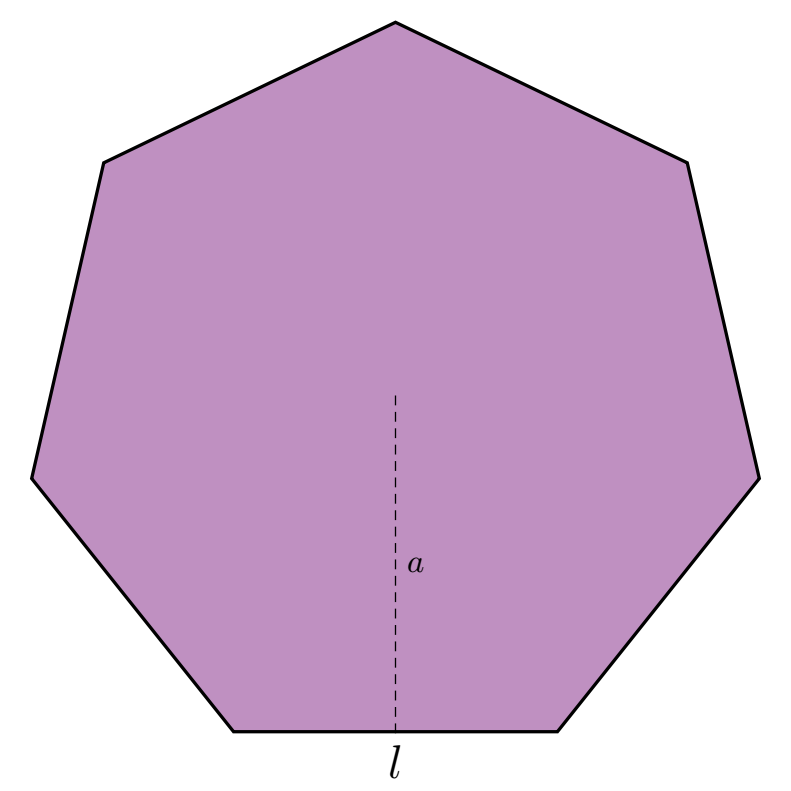
\includegraphics[width=0.6\linewidth]{mexmat00005.png}\\
                                    Perímetro: \fillin[84][0.3in] \quad Área: \fillin[378][0.3in]
                              }
                        \begin{solutionbox}{3cm}
                        \end{solutionbox}

                        % \part Si la base mayor del trapecio mide 33, su base menor 12 y su altura 14.
                        % 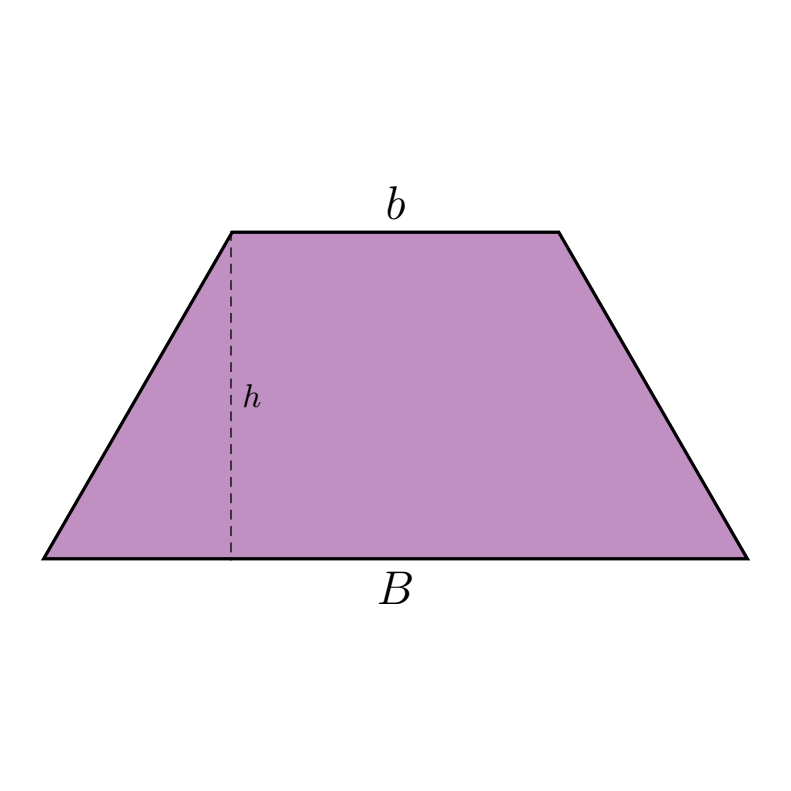
\includegraphics[width=0.9\linewidth]{mexmat00006.png}\\
                        % Área: \fillin[][0.3in]

                        % \begin{solutionbox}{1.5cm}
                        % \end{solutionbox}

                        \part Si el lado del pentágono mide 25 y su apotema 18.

                              {\centering
                                    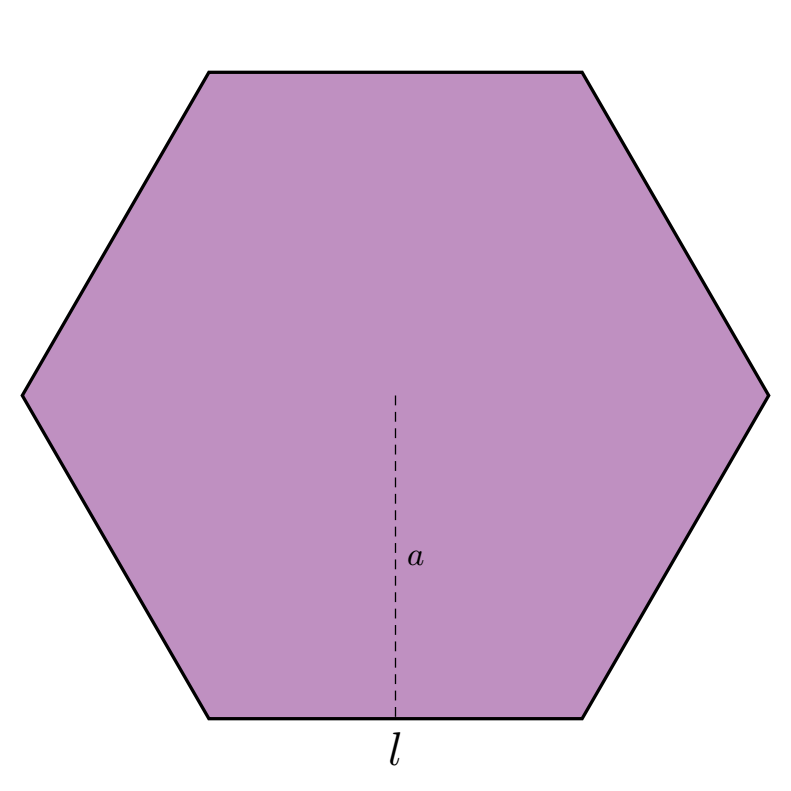
\includegraphics[width=0.6\linewidth]{mexmat00007.png}\\
                                    Perímetro: \fillin[][0.3in] \quad Área: \fillin[][0.3in]
                              }
                        \begin{solutionbox}{3cm}
                        \end{solutionbox}


                  \end{parts}
            \end{multicols}
      }

      \newpage
      \subsection*{Área lateral,área total y volumen}


      \question[6]{Calcula el volumen, el área lateral y el área total de las siguientes figuras:

            % \begin{multicols}{2}
            %       \begin{parts}
            %             \part 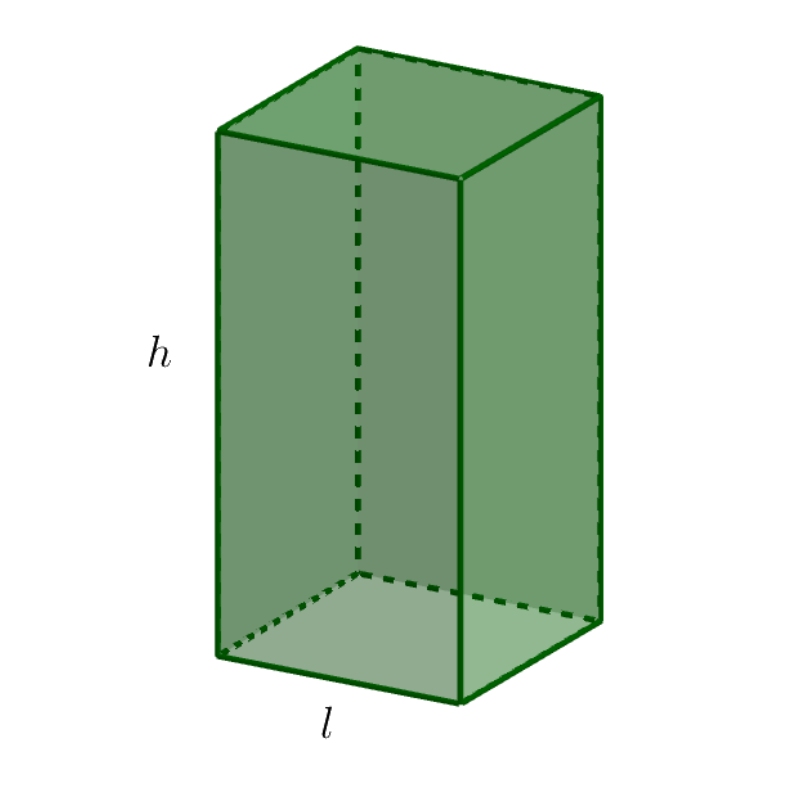
\includegraphics[width=0.65\linewidth]{mexmat00008.png}\\
            %             Prisma cuyos lados "l" de la base miden 15 cm y la altura "h" mide 24 cm.

            %             Área Lateral: \fillin[][0in]

            %             \begin{solutionbox}{1cm}
            %             \end{solutionbox}

            %             Área Total: \fillin[][0in]

            %             \begin{solutionbox}{1cm}
            %             \end{solutionbox}

            %             Volumen: \fillin[][0in]

            %             \begin{solutionbox}{1cm}
            %             \end{solutionbox}

            \begin{multicols}{2}
                  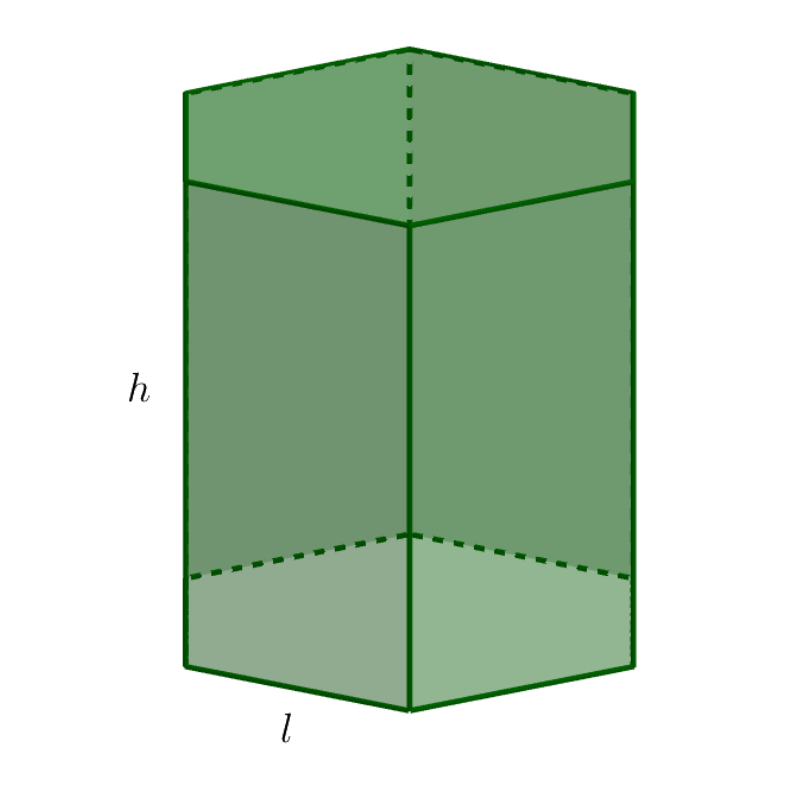
\includegraphics[width=0.7\linewidth]{mexmat00009.png}\\

                  \columnbreak%

                  Prisma cuyos lados "l" de la base miden 15.2 cm, el apotema mide 12.5 y la altura "h" mide 41.4 cm.

                  Área Lateral: \fillin[][0in]

                  \begin{solutionbox}{1cm}
                  \end{solutionbox}

                  Área Total: \fillin[][0in]

                  \begin{solutionbox}{1cm}
                  \end{solutionbox}

                  Volumen: \fillin[][0in]

                  \begin{solutionbox}{1cm}
                  \end{solutionbox}

            \end{multicols}


            %       \end{parts}
            % \end{multicols}
      }

\end{questions}
\end{document}